\documentclass[journal, 10pt]{IEEEtran}
% *** CITATION PACKAGES ***
%
\usepackage{cite}
% cite.sty was written by Donald Arseneau
% V1.6 and later of IEEEtran pre-defines the format of the cite.sty package
% \cite{} output to follow that of IEEE. Loading the cite package will
% result in citation numbers being automatically sorted and properly
% "compressed/ranged". e.g., [1], [9], [2], [7], [5], [6] without using
% cite.sty will become [1], [2], [5]--[7], [9] using cite.sty. cite.sty's
% \cite will automatically add leading space, if needed.
\usepackage{amssymb}

% *** GRAPHICS RELATED PACKAGES ***
%
\ifCLASSINFOpdf
  \usepackage[pdftex]{graphicx}
\else
   \usepackage[dvips]{graphicx}
    % \DeclareGraphicsExtensions{.eps}
\fi
\usepackage{graphicx}

% *** MATH PACKAGES ***
\usepackage[cmex10]{amsmath}
% Also, note that the amsmath package sets \interdisplaylinepenalty to 10000
% thus preventing page breaks from occurring within multiline equations. Use:
%\interdisplaylinepenalty=2500 after loading amsmath to restore such page breaks as IEEEtran.cls normally

% *** ALIGNMENT PACKAGES ***
\usepackage{array}

% *** SUBFIGURE PACKAGES ***
\ifCLASSOPTIONcompsoc
  \usepackage[caption=false,font=normalsize,labelfont=sf,textfont=sf]{subfig}
\else
  \usepackage[caption=false,font=footnotesize]{subfig}
\fi
 %subfig.sty
% *** FLOAT PACKAGES ***
%\usepackage{float}
\usepackage{stfloats}

\begin{document}
\title{Virtual Simulation for Testing a Vision-Based Autonomous Docking and Navigation Algorithm}
%
% use \thanks{} to gain access to the first footnote area
% a separate \thanks must be used for each paragraph as LaTeX2e's \thanks
% was not built to handle multiple paragraphs
%
\author{John Karasinski, Christopher Lorenzen, and Melanie Stich\\Department of Mechanical \& Aerospace Engineering\\University of California, Davis\\Davis, CA, USA }

% The paper headers
%\markboth{Journal of \LaTeX\ Class Files,~Vol.~11, No.~4, December~2012}%
%{Shell \MakeLowercase{\textit{et al.}}: Bare Demo of IEEEtran.cls for Journals}

\maketitle

% As a general rule, do not put math, special symbols or citations
% in the abstract or keywords.
\begin{abstract}
The abstract goes here.
\end{abstract}

% Note that keywords are not normally used for peerreview papers.
\begin{IEEEkeywords}
robots, satellite
\end{IEEEkeywords}


\section{Introduction}

This demo file is intended to serve as a ``starter file''
for IEEE journal papers produced under \LaTeX\ using
IEEEtran.cls version 1.8 and later.

I wish you the best of success.

\subsection{Background}
Subsection text here.

\subsection{Motivation}
Motivation here

\subsection{Objective}
What is our specific question?

\subsection{Outline}
Don't know if we want this section, but just copied it over from Joshi's example paper.


% An example of a double column floating figure using two subfigures.
% (The subfig.sty package must be loaded for this to work.)
% The subfigure \label commands are set within each subfloat command,
% and the \label for the overall figure must come after \caption.
% \hfil is used as a separator to get equal spacing.
% Watch out that the combined width of all the subfigures on a
% line do not exceed the text width or a line break will occur.
%
%\begin{figure*}[!t]
%\centering
%\subfloat[Case I]{\includegraphics[width=2.5in]{Penguins}%
%\label{fig_first_case}}
%\hfil
%\subfloat[Case II]{\includegraphics[width=2.5in]{Penguins}%
%\label{fig_second_case}}
%\caption{Simulation results.}
%\label{fig_sim}
%\end{figure*}
%%

%\begin{table}[!t]
%% increase table row spacing, adjust to taste
%\renewcommand{\arraystretch}{1.3}
%% if using array.sty, it might be a good idea to tweak the value of
%% \extrarowheight as needed to properly center the text within the cells
%\caption{An Example of a Table}
%\label{table_example}
%\centering
%% Some packages, such as MDW tools, offer better commands for making tables
%% than the plain LaTeX2e tabular which is used here.
%\begin{tabular}{|c||c|}
%\hline
%One & Two\\
%\hline
%Three & Four\\
%\hline
%\end{tabular}
%\end{table}

\section{Literature Review}
\subsection{SPHERES Vertigo}

\subsection{Anti-Collision Algorithms}

\subsection{Visual Simulations}

\clearpage
\section{The Environment}
\subsection{The Spacecraft Environment}
Space is an extremely dangerous environment with many challenges of different natures and magnitudes. Some effects on spacecraft can arise from radiation, space debris and meteoroid impact, upper atmospheric drag, spacecraft electrostatic charging, and many other factors. While the resulting dynamics of these phenomena have various degrees of effect on small spacecraft, these are outside the scope of this work. For the purposes of the study, all of these factors are ignored. It is assumed here that the spacecraft is operating under nominal conditions in an otherwise empty environment.

\subsection{Dynamical Equations of Motion}
\label{cweqs}
The Clohessy-Wiltshire equations were used to model the dynamics of the spacecraft while it was in close proximity to the target vehicle. The Clohessy-Wiltshire equations describe a simplified model of orbital relative motion, in which the target is in a circular orbit, and the chaser spacecraft is in an elliptical or circular orbit. This model gives a first-order approximation of the chaser's motion in a target-centered coordinate system. It is used here in planning rendezvous of the chaser with the target~\cite{cw_eqs}.

These equations of motion can be expressed as
\begin{equation}
\begin{split}
\ddot{x} &= 3n^2 + 2n\dot y \\
\ddot{y} &= -2n\dot x \\
\ddot{z} &= -n^2z
\end{split}
\end{equation}
and have the closed form solution given by
\begin{equation}
\begin{split}
x(t) = (4-3 \cos{nt})x_0 &+ \frac{sin{nt}}{n}\dot x_0 + \frac{2}{n} (1 - \cos(nt))\dot y_0\\
y(t) = 6(\sin{nt}-nt)x_0 &+ y_0 \frac{-2}{n}(1 - \cos{nt})\dot x_0 \\
                         &+ \frac{4 \sin{nt} - 3nt}{n}\dot y_0 \\
z(t) = z_0 \cos{nt} &+ \frac{\dot z_0}{n} \sin{nt}
\end{split}
\end{equation}
where
\begin{equation}
n = \sqrt{\frac{\mu}{a^3_t}}
\end{equation}
and $a_t$ is the semi-major axis of the target vehicle's orbit and $\mu$ is the standard gravitational parameter.

\section{Simulation}
The virtual simulation was driven with a variety of software packages. The dynamics and control systems were driven by several Python modules, while the visualization was rendered in EDGE. EDGE is a graphics display tool developed at NASA's Johnson Space Center that combines key elements from graphics software developed for the space shuttle and the International Space Station programs and adapts them for integration with other engineering simulations and facilities~\cite{EDGE}.

EDGE makes use of a node tree to structure data, objects, and models. Each node has many properties, the most notable of which are position, orientation, and the node's parent. Each node's position and orientation are defined relative to it's parent's position and attitude. A node's parent can be changed to a different node, at which time the node's position and attitude are automatically updated to the correct values.

Three Python Python 2.7.9 scripts were developed for use in the virtual simulation:
\begin{description}
    \item[\textbf{\textit{cv}}] \hfill \\
    A computer vision image processing module which takes advantage of OpenCV-Python version 2.4.9.
    \item[\textbf{\textit{dynamics}}] \hfill \\
    A dynamics and controls module.
    \item[\textbf{\textit{dcomm}}] \hfill \\
    A wrapper library developed to interface with EDGE's C++ DCOMM library.
\end{description}

\subsection{Python Modules}
\begin{figure}[tbh]
\begin{center}
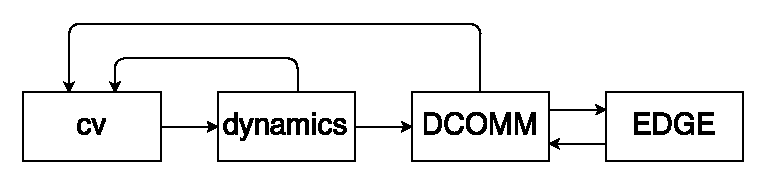
\includegraphics[width=0.5\textwidth]{figures/block.pdf}
\caption{Block diagram of software package interactions}
\label{c1_plot}
\end{center}
\end{figure}

\subsubsection{cv}
The \textit{cv} module takes advantage of Python bindings for OpenCV. OpenCV (Open Source Computer Vision) is a library of programming functions mainly aimed at real-time computer vision. This module takes the live video feed from EDGE and attempts to identify features visible on the target spacecraft. The features of the target are supplied to the module a priori, and these descriptions were used to estimate the 3D pose of the target vehicle relative to the spacecraft's camera. This pose information is passed on to the \textit{dynamics} module

\subsubsection{dynamics}
The \textit{dynamics} module drives the dynamics and control of the simulation. The movement of the spacecraft around the target craft is modeled by the Clohessy-Wiltshire equations, see section~\ref{cweqs}. This module controls how the spacecraft operated in its different modes. Depending on pilot input, the spacecraft can navigate purely on line of sight, laser guided sensors to approach and hold a distance from a target, make use of the optical camera and machine vision to identify and dock with docking ports, or display guidance for a human pilot.

\subsubsection{DCOMM}
The \textit{DCOMM} module was previously developed to network between Python scripts and EDGE. The Python DCOMM interface allows a user to call various C++ functions from EDGE's DCOMM module and communicate with an EDGE server. Users can move and rotate nodes, and can also change a node's parents, units, and principal axis definitions. Commands to set the spacecraft's attitude and position were sent from the \textit{dynamics} module through DCOMM and passed on to EDGE. This module was also responsible for requesting and handing off the video feed from the EDGE server.

\clearpage

\section{Architectures}
Use this section to describe which Joshi-defined architecture was implemented for our simulation (ie. Reactive, Deliberative Architecture, or both)
**** DOES THIS SECTION WAIT TILL THE FINAL PAPER??

\section{Techniques and Algorithms}
not sure if this section should only be used for the final paper

%final paper only
%\section{Simulation Results and Discussion}

\section{Conclusion}
The conclusion goes here.

%final paper only
%\section{Future Work}

\nocite{*}
\bibliographystyle{ieeetr}
\bibliography{MAE252_MT_StichLorenzenKarasinski}{}

\end{document}
